\documentclass[a4paper,10pt,toc=graduated]{article}
\usepackage[utf8]{inputenc}
\usepackage[toc,page]{appendix}
\usepackage[margin=2.5cm]{geometry}
\usepackage{amssymb}
\usepackage{listings}
\usepackage{graphicx}

\newcommand{\tab}{\hspace*{2em}}
\newenvironment{answer}{
 \begingroup
 \bf
 \small
}{
 \endgroup
 \bigskip
}

\newenvironment{mysection}
{
\begin{center}
\begin{em}
\bf
}
{
\end{em}
\end{center}
}

\newenvironment{mysection2}[1]
{
\begin{center}
\begin{em}
\bf
\large
 #1
\end{em}
\end{center}
}
{
}

\newenvironment{mySubsection}[1]
{
\begin{flushleft}
 \bf
 \uppercase{
 #1
 }
\end{flushleft}
}
{
}
\usepackage{lastpage}
\usepackage{fancyhdr}
\pagestyle{fancy}

\lhead{}
\chead{}
\rhead{}
\lfoot{}
\cfoot{Version 1.0}
\rfoot{Page \thepage\ of \pageref{LastPage}}
\lfoot{
 Last Updated:
 \today
}
\renewcommand{\headrulewidth}{0pt}
\renewcommand{\footrulewidth}{0pt}

\setlength{\headheight}{0pt}

\newcommand*\myFirstPageHeader{
  \begingroup
  \flushright
  \docauthor

  \begin{center}
  \Large
  \doctitle
  \end{center}
  
  \endgroup
}
  



\newcommand*\docauthor{
Josh Gillham
\\
Randy Mangel
\\
Sann Voun
\\
Daniel Eason
\\
}
\newcommand*\doctitle{The Weekly Meal Planner}
\newcommand*\className{CS3810}

\author{\docauthor}
\title{\doctitle}

\begin{document}
\vspace*{\fill}

\begin{center}
\begin{em}
\bf
\huge
\noindent
\uppercase{
\doctitle
}

\large
Data Base Design Document (DBDD)

\end{em}
\end{center}
\vspace{\fill}

\begin{center}
\tiny
By

\begin{em}
\small
\noindent
\uppercase{
\docauthor
}
\end{em}
\end{center}
\vspace{\fill}


\newpage
\setcounter{tocdepth}{2}
\tableofcontents
\newpage
\section{Introduction}
\begin{mySubsection}{Motivation}
People around the world with full time schedules may find themselves too busy
to plan their meals.
Other people not so busy find planning meals inconvenient.
Both people may find themselves using fast food services
or simply skipping meals.

There are people who would like to eat regular meals throughout the day
and have the taste of home-style cooking.
There are people who would like a method to easily total nutritional daily in-take.
For example, fats, calories, sodium, and many more.
There are people who would like to be introduced to new meals every day.
There are people who would like to have a shopping list printed for them.

Young adults in college could benefit from a meal planner service.
They need help adding nutrition to their diets
while controlling their calories and fats.
They need to know what to buy at the store.
They would love to try new foods too.
A service could help by
adding nutrition,
creating shopping lists,
and introducing them to new foods.

Young single mothers have busy lives of balancing work and parenting.
Left over time is scarce.
Since making home cooked meals requires much preparation time,
they would benefit from a service
that tells them what to buy at the store
and otherwise chooses meals for them based off past favorites.

All people would love to cut down on the time required to plan meals
and gain more variety in their diets.
They would rather not think about what they need on shopping lists.
\end{mySubsection}

\begin{mySubsection}{Service Definition}
The Weekly Meal Planner service assists customers with planning their meals.
The service will provide the customer with
the opportunity to try new meals daily
while avoiding food allergies
and staying on track with dietary plans.
For example, a customer could prefer vegetarian or glutean-free meals only.
Customers will be provided with their own user account.
The user account will give them the convenience of access to the service
from virtually any where.
The account will allow the user to save their daily meal plans
as well as their dietary preferences.
The account will allow the user to elect a list of favorite meals.
\end{mySubsection}
\begin{mySubsection}{Defining the Audience}
\noindent
The weekly meal planner is a service designed to serve anyone and everyone.
The service interfaces with the customer via a website or mobile application.
These interfaces will give customers world-wide access to the service.
\newline
\end{mySubsection}

\begin{mySubsection}{Features}
\begin{itemize}
\item Avoids the user's disliked meals.
\item Encourages the user's liked meals.
\item Stores the user's favorite meals.
\item Introduces customers to new meals.
\item Prints a shopping list for a date range.
\item Avoids meals by characteristic, for example, "no cheese."
\item Avoids meals by recommendations set forth by a dietition.
\end{itemize}
\end{mySubsection}


\section{Assumptions/Risks/Constraints}
\begin{mySubsection}{Assumptions}
Assumptions were made to simplify the design.
The designers may decide to add and remove assumptions
as the project goals change.
\begin{enumerate}
\item The meal ingredients and directions will apply to only one person.
\item The user will not want to customize their meal plan.
\item The user will not need to know the name of the store where an ingredient may be sold.
\item The user will not want a list of favorite meals.
\end{enumerate}
\end{mySubsection}
\begin{mySubsection}{Risks}
\begin{enumerate}
\item After producing the DDL for a target database, transitioning to new technology will be costly.
\item The customer base may be smaller than expected.
\item Some competitors may be hard to compete against.
\end{enumerate}
\end{mySubsection}
\section{Design Decisions}
\begin{mySubsection}{Influencing Factors}
\begin{enumerate}
\item The Weekly Meal Planner comes from our own personal experiences.
\item Randy Mangel was instrumental in providing us with this idea.
\end{enumerate}
\end{mySubsection}
\begin{mySubsection}{Tools}
\begin{enumerate}
\item Java JDK 1.6-7
\item Oracle Database
\item Oracle SQL Developer 3
\item Oracle SQL Data Modeler 3
\item Netbeans 7.3.1
\item Microsoft Paint
\item Vi/Vim
\item UNIX Bash Scripts
\end{enumerate}
\end{mySubsection}
\begin{mySubsection}{CONOPS}
\noindent
There will be three different types of users: limited, doctor, and admin.
Each user will play a different role.
The limited user will consume the service but will not have the power to prescribe dietary recommendations.
The doctor will have all the abilities of the limited user but will also be able to prescribe dietary recommendations.
The admin user will not be limited.
The admin will be responsible for maintaining the database, correcting errors, and will be used by developers.
\newline

\noindent
The service will be a meal management and scheduling tool for limited user.
The limited user may find meals in the catalog.
They may rate, favorite, or select meals.
They may rate meals on a scale of 0 to 5 stars.
They may add the meal to the list of their favorites.
They may select meals and schedule a meal for a particular day and time (morning, noon, afternoon, and evening).
\newline

\noindent
The limited user will use the tool to track their meal schedule.
The user will be able to see a calendar showing their meal plans.
The user may delete or replace meals on their schedule.
\newline

\noindent
The limited user will use the tool to generate a shopping list.
The shopping list will help the user estimate the cost of food and help them find stores where the item might be sold.
\newline

\noindent
The limited user will also use the tool to find the recipe with step-by-step preparation instructions.
\newline

\noindent
The doctor user will be able to prescribe dietary recommendations for a set of users.
\end{mySubsection}
\begin{mySubsection}{Primary Project Requirements}
\renewcommand{\labelenumi}{\arabic{enumi}. }
\renewcommand{\labelenumii}{\arabic{enumi}.\arabic{enumii}. }
\renewcommand{\labelenumiii}{\arabic{enumi}.\arabic{enumii}.\arabic{enumiii}. }
\renewcommand{\labelenumiv}{\arabic{enumi}.\arabic{enumii}.\arabic{enumiii}. }
\renewcommand{\labelenumiv}{\arabic{enumi}.\arabic{enumii}.\arabic{enumiii}.\arabic{enumiv}. }

\begin{enumerate}
\item
There will be a relation of meals.
\begin{enumerate}
\item
Each meal will have a minimum of 1 course.
\begin{enumerate}
\item
A course will have a name.
\item
A course is a dish or sub-meal that represents one type of food.
\item
Each course will have ingredients.
\begin{enumerate}
\item
Ingredients will have a name.
\item
Each ingredient will have a serving size, calorie count, and fat count.
\end{enumerate}
\end{enumerate}
\end{enumerate}
\item
There will be a relation of users.
\begin{enumerate}
\item
Each user will have a user name, First and last name, and email address.
\item
Each user may have many meal plans (usually not more than 3 or less than 1) per day.
\begin{enumerate}
\item
A meal plan (or called user selected meals) is a list of meals per day per user.
\end{enumerate}
\item
Each user will have a list of favorite meals.
\item
Each user will have an optional rating per meal.
\item
The system will determine the average rating per meal.
\end{enumerate}
\item
There will be a GUI.
\begin{enumerate}
\item
The GUI will be a set of views. Where each view is tailored to the activity.
\begin{enumerate}
\item
The user type may be “limited”, "dietition", or may be “admin”.
\begin{enumerate}
\item
“limited” types will be limited on which activities they can interact with.
This type will be able to have daily meal plans, a favorite meals list,
and set dietary preferences.
This type will be allowed to print shopping lists as well.
\item
"dietition" types will like a "limited" user
only with the ability to prescribe dietary recommendations for other users.
\item
“admin” types will have no limits on which activities they can interact with.
The primary role will be in maintaining and correcting errors in the database.
\end{enumerate}
\item
Each activity will take a specific action on the database or obtain results.
\begin{enumerate}
\item
Find Meals: this activity will allow the user to find a meal from the list of available meals.
\item
View Meal Plan: this activity will allow the user to add, remove, rate, and favorite meals.
\item
View/Print Shopping List: this allows the user to generate and print a shopping list for day’s or a set of days’ meal plans.
\end{enumerate}
\end{enumerate}
\end{enumerate}
\end{enumerate}
\end{mySubsection}
\begin{mySubsection}{Data Requirements}
\begin{itemize}
\item
Each meal will consist of Preparation instructions, Ingredients, a shopping list, an adjustable serving size, and a price range. Any customer will be able to query the meals by price range in order for them to be able to stay within a certain budget.
\item
Each Customer will have their own ID, name, password, security questions and address. They will also have a list of favorite meals along with a list of meals they do not like.
\item
There will also be a list of meals that are gluten free and or vegetarian. These meals will be stored within the other meals but will only be displayed if they are specifically requested by the customer.
\item
Each meal will have a rating generator that will come from the rating from each customer and be averaged to create an overall rating.
\end{itemize}
\end{mySubsection}
\begin{mySubsection}{Users}
\renewcommand{\labelenumi}{}
\renewcommand{\labelenumii}{}
\begin{enumerate}
\item {[limited]}
This user can consume the service, but, not perform any administrative or doctoral actions. The user may browse the meal catalog, rate meals, favorite meals, view/print shopping lists, and view/print weekly meal schedule.

\item {[doctor]}
This user can consume the service like the limited user, but, can also prescribe a diet recommendation to a specific user.

\item {[admin]}
This user has no limitations accessible activities.
\end{enumerate}
\end{mySubsection}
\begin{mySubsection}{Functional Requirements}
There are four types of processes that are relevant:
\renewcommand{\labelenumi}{}
\renewcommand{\labelenumii}{}
\begin{enumerate}
\item
Limited User
\begin{enumerate}
\item {[Browse]}
This process allows customers to query the database to find certain meals. The customer may select a meal and add that meal to their daily meal plan.
\item {[Favorite]}
This process takes a meal out of the big list of meals and places it into the customers favorite list.
\item {[Unfavorite]}
This process removes the meal from the customers favorite list.
\item {[Rate]}
This process will allow the users to rate the meals which will allow the administrators to keep track of meals that people are enjoying along with ones that are not doing very well.
\end{enumerate}
\item Dietitian User
\begin{enumerate}
\item {[Prescribe]}
This process allows the doctor to make a dietary recommendation.
\end{enumerate}
\item
Admin User
\begin{enumerate}
\item {[admin]}
This process modifies the database information about customers and or meals.
\end{enumerate}
\end{enumerate}
\end{mySubsection}
\begin{mySubsection}{Business rules}
\renewcommand{\labelenumi}{}
\renewcommand{\labelenumii}{\arabic{enumii}. }
\begin{enumerate}
\item
Dietitians
\begin{enumerate}
\item
Only doctors may prescribe a dietary recommendation.
\item
Meals
\item
Meals will be  allowed in three categories: Regular, Gluten-free, Vegetarian. 
\item
Each customer will be allowed to customize their meal choices using those three options. 
\item
Decisions for each weeks meal plan will be made based upon the ratings collected from the customers
\item
Each meal will be set to a 2 serving default, which can be changed by the user.
\end{enumerate}
\item
Customers
\begin{enumerate}
\item
Customers must create their own personal log in in order to use the like and dislike feature of the meals.
\item
Customers can never see more than a weeks worth of meals in order to limit their access to the meals
Meals put on the customers dislike list will be banned from returning to that users weekly meal plan. If a meal in the administrative weekly plan conflicts with the users dislike list a replacement meal will be provided for the customer. 
\item
A user shall have a limit of no more than 3000 calories per day in meals.
\item
A user shall be given exactly 3 meals for a day.
\item
A user shall not be given meals that go against the limitations set by their dietitian.
\end{enumerate}
\item
Ratings
\begin{enumerate}
\item
Ratings will be updated after each week, and will be a major determining factor in the administrators decisions about the meal schedule each week.
\end{enumerate}
\item
Updates
\begin{enumerate}
\item
Users will be allowed to recommend new recipes to the administrators 
\end{enumerate}
\end{enumerate}
\end{mySubsection}
 
 
\begin{mySubsection}{Screens}
\renewcommand{\labelenumi}{\arabic{enumi}. }
\renewcommand{\labelenumii}{\arabic{enumi}.\arabic{enumii}. }
\renewcommand{\labelenumiii}{\arabic{enumi}.\arabic{enumii}.\arabic{enumiii}. }
\renewcommand{\labelenumiv}{\arabic{enumi}.\arabic{enumii}.\arabic{enumiii}. }
\renewcommand{\labelenumiv}{\arabic{enumi}.\arabic{enumii}.\arabic{enumiii}.\arabic{enumiv}. }
\begin{enumerate}
\item
Main screen
\begin{enumerate}
\item
Login
\item
Create new user
\end{enumerate}
\item
Home Screen
\begin{enumerate}
\item
List of meals for the week
\begin{enumerate}
\item
Each meal will have thumbs up or thumbs down which are clickable.
\end{enumerate}
\item
Settings button
\item
Filter button
\begin{enumerate}
\item
Price
\item
Meal type
\item
Meal ingredients(chicken, Steak… etc..)
\end{enumerate}
\item
Log out Button
\end{enumerate}
\end{enumerate}
\end{mySubsection}
\begin{mySubsection}{What we learned}
\begin{enumerate}
\item
How to write SQL statements.
\item
How to use Oracle SQL Data Modeler.
\item
How to use Spiral Development.
\end{enumerate}
\end{mySubsection}
\section{Detailed Data Base Design}
\begin{mySubsection}{Entities}
\begin{enumerate}
\item Attributes
-- Defines attributes by name.
\item Courses
-- Defines courses by name with the servings.
\item DayPlans
-- Deprecated.
\item Dietition
-- Defines users with elevated permissions.
They differ from standard users only in that they can prescribe dietary
recommendations.
\item Emails
-- Defines emails per user.
Each email is unique to a user.
\item Ingredients
-- Defines ingredients by name.
For example,
cooking items such as salt, pepper, oil, eggs, and wafles are all ingredients.
\item IngredientsCourses
-- Defines a relationship between ingredients and courses.
There are two attributes corresponding to the public keys of
each table respectively, of course.
\item Meals
-- Defines meals by names.
Meals are made of courses.
For example,
the American breakfast consists of eggs, bacon, and sausage.
\item UserSelectedMeals
-- Defines meals that appear on a user's schedule for a specific day.
\item MealsCourses
-- Defines the many to many relationship between meals and courses.
\item MealsFoodAttributes
-- Defines the many to many relationship between meals and attributes.
\item Prescription
-- Defines a dietary description for a user and made on a certain date.
\item PrescriptionAttributes
-- Defines a many to many relationship between prescription and attributes.
\item Ratings
-- Defines a many to many relationship between users and meals with a rating from 0 to 5 stars.
\item UserType
-- Defines different types of users.
We are not sure of the user for this, yet.
This table maybe deprecated.
\item Users
-- Defines a user with a first name, last name, user name, gender,
password, and user type.
The user type attribute may be deprecated soon.

\end{enumerate}

\end{mySubsection}
\section{Design Process}
\begin{mySubsection}{Automated Processing of Data Modeler DDL Output}
We saw that the SQL generated by Data Modeler was missing some key features. We needed the DDL code to add drop code prior to creation code to ensure that designs were getting refreshed. The following script automates the process of adding drop code per creation code.
\newline
\end{mySubsection}
\section{Java Application Design}
We tried to map the classes in the program to each phase of the user story.
For example, the user must first login using the FormLogin
or register an account using the FormRegistration.
This technique, called domain-driven design (DDD),
tries to map each class in the program to the user activity
as first described by Eric Evans.
\newline

\makebox[\textwidth]{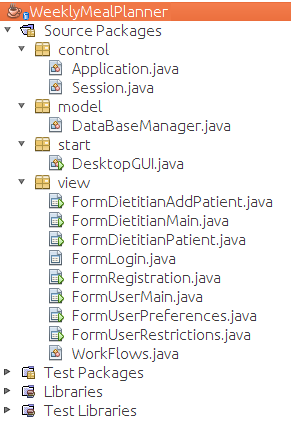
\includegraphics[width=8cm]{figures/ProjectHierarchy.png}}

As seen in the figure above,
the program code is divided into four packages: control, model, start, view.
Each package is directly related to its responsibillity.
For example,
the control package contains application logic prevent more than one user login
from being active during the application life cycle.
The view package contains code related to displaying user forms.
The model package contains code related to talking to the data base.

\section{Development Cycle}
\subsection{Description}
We are using the spiral development model.
Using this model,
we will group subsets of features into a meta-goals called a milestone.
Each milestone will not have all project features.

\makebox[\textwidth]{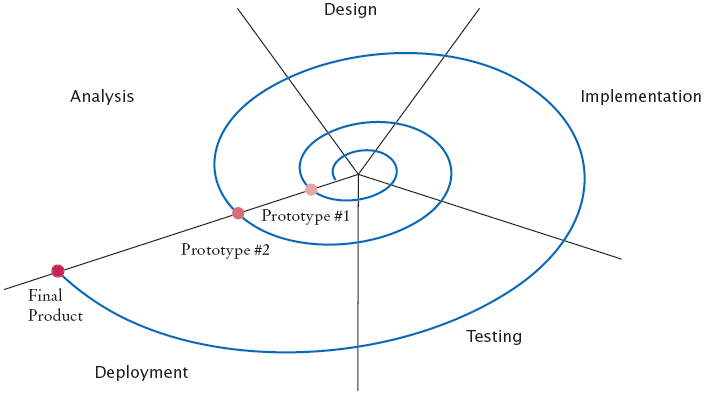
\includegraphics[width=8cm]{figures/SpiralDevelopment.png}}

\subsection{Current Status}
We have made progress in all areas: DDL, testing, and the Java application.
The DDL is nearly complete.
All tables have been completed.
The primary key and the foreign constraints still need to be added.
\newline

With our insertion data,
we feel confident that the design is behaving as we expect.
We need to test again after all the constraints have been added.
\newline

The Java application is showing great progress.
The user can list meals, courses, ingredients, and nutritional facts.
The user cannot yet set preferences or view dietary restrictions.
\newline

The application does not have all roles implemented.
The dietition currently cannot perform his role.
The admin currently cannot perform his role as well.

\newpage
\begin{appendices}
\section{Data Base Design}
\subsection{Logical Model}
\begin{center}
  \makebox[\textwidth]{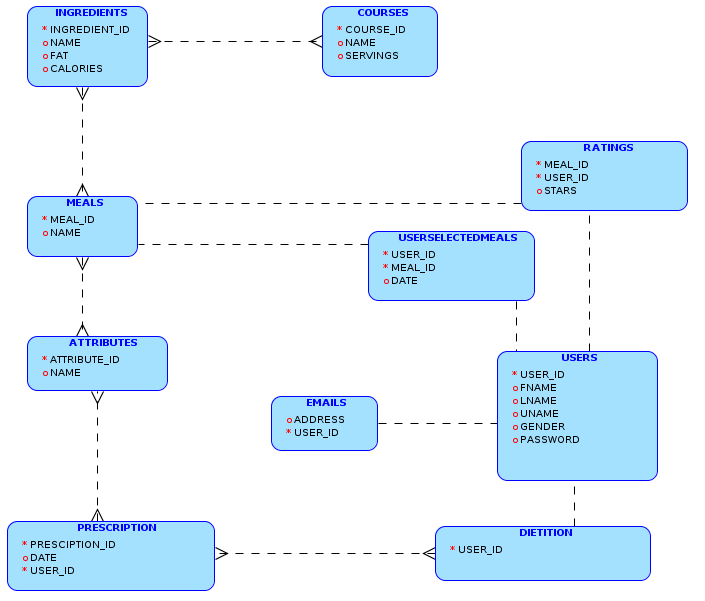
\includegraphics[width=\paperwidth]{figures/LogicalModel.png}}
\end{center}
\subsection{Relational Model}
\begin{center}
  \makebox[\textwidth]{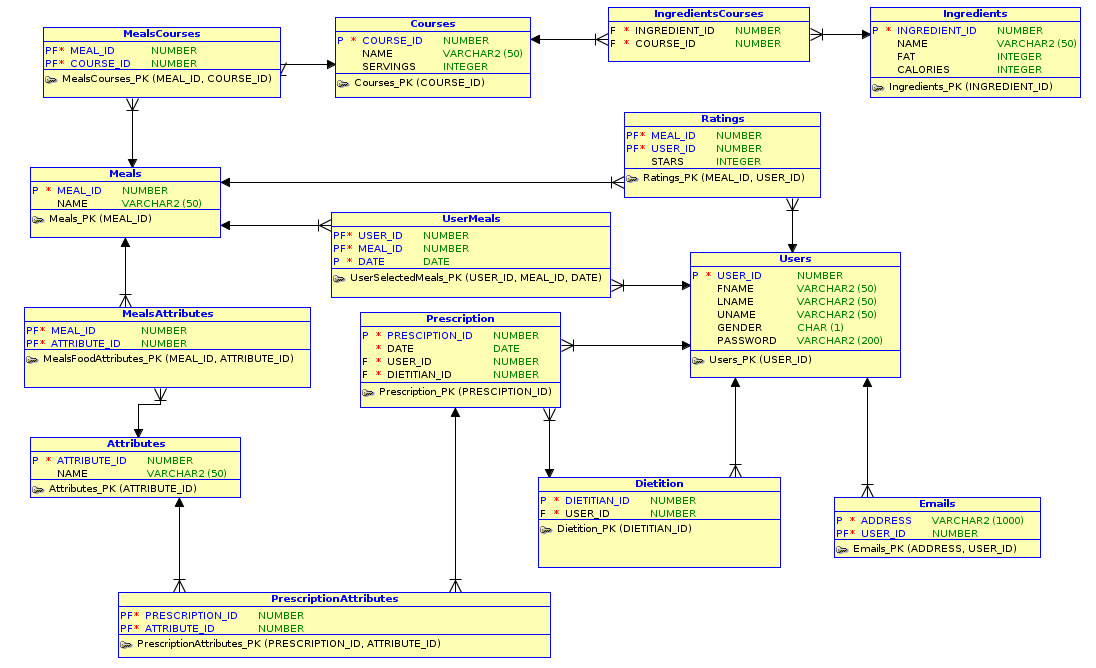
\includegraphics[width=\paperwidth]{figures/RelationalModel.png}}
\end{center}
\section{Java Application GUI}
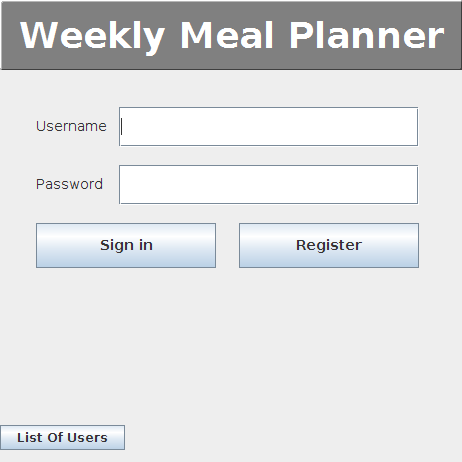
\includegraphics{screenshots/frmLogin.png}

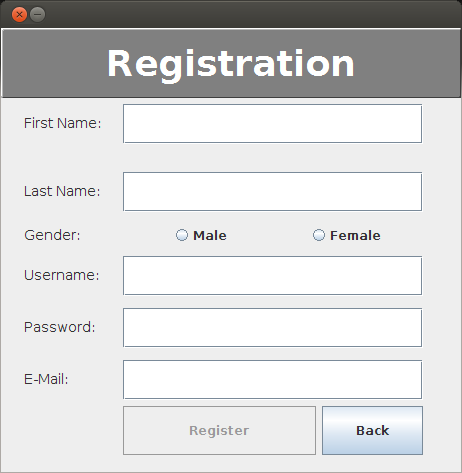
\includegraphics{screenshots/frmRegistration.png}

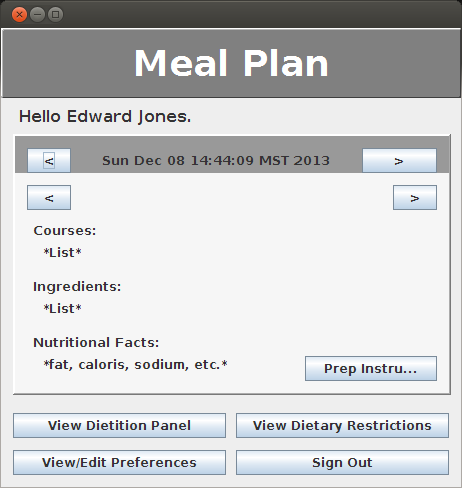
\includegraphics{screenshots/frmUserMain.png}

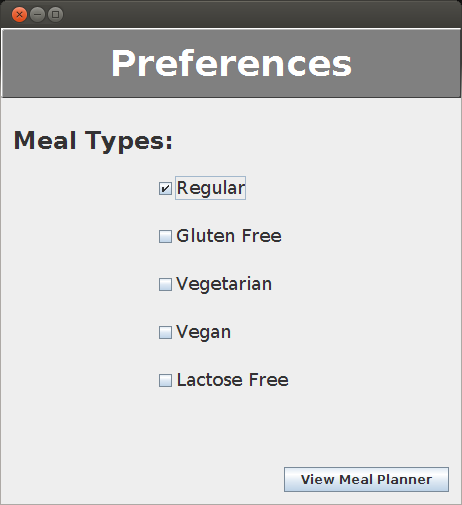
\includegraphics{screenshots/FormUserPreferences.png}

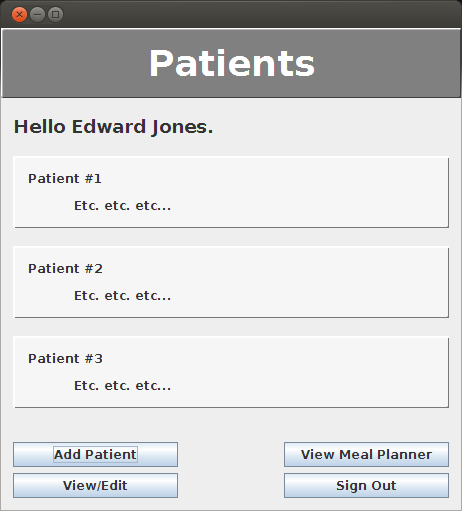
\includegraphics{screenshots/frmDietitionMain.png}
\section{Bash Scripts}
\begin{mySubsection}{Data Modeler to SQL Conversion}
\lstinputlisting[language=bash]{../ddl/conv.sh}
\end{mySubsection}
\begin{mySubsection}{Data Design Language}
\lstinputlisting[language=SQL]{../ddl/Tables.sql}
\end{mySubsection}
\section{Testing}
\begin{mySubsection}{Data Insertion}
\lstinputlisting[language=SQL]{../test-data/Insertion.sql}
\end{mySubsection}
\section{Java Source code}
\input{gen/java-source-listing.tex}
\section{Source Code Line Count Report}
\lstinputlisting{gen/source-line-count.txt}
\end{appendices}

\end{document}
